%!TEX root=./user_guide.tex
\chapter{Code Overview}
\wannier\ can operate in two modes:

\begin{enumerate}
\item {\it Post-processing mode:} read in the overlaps and projections
  from file as computed inside a first-principles code. We expect this
  to be the most common route to using \wannier, and is described in
  Ch.~\ref{ch:wann-pp};


\item {\it Library mode:} as a set of library routines to be called
  from within a first-principles code that passes the overlaps and
  projections to the \wannier\ library routines and in return gets the
  unitary transformation corresponding to MLWF. This route should be
  used if the MLWF are needed within the first-principles code, for
  example in post-LDA methods such as LDA+U or SIC, and is described
  in Ch.~\ref{ch:wann-lib}.
\end{enumerate}


\begin{figure}
\begin{center}
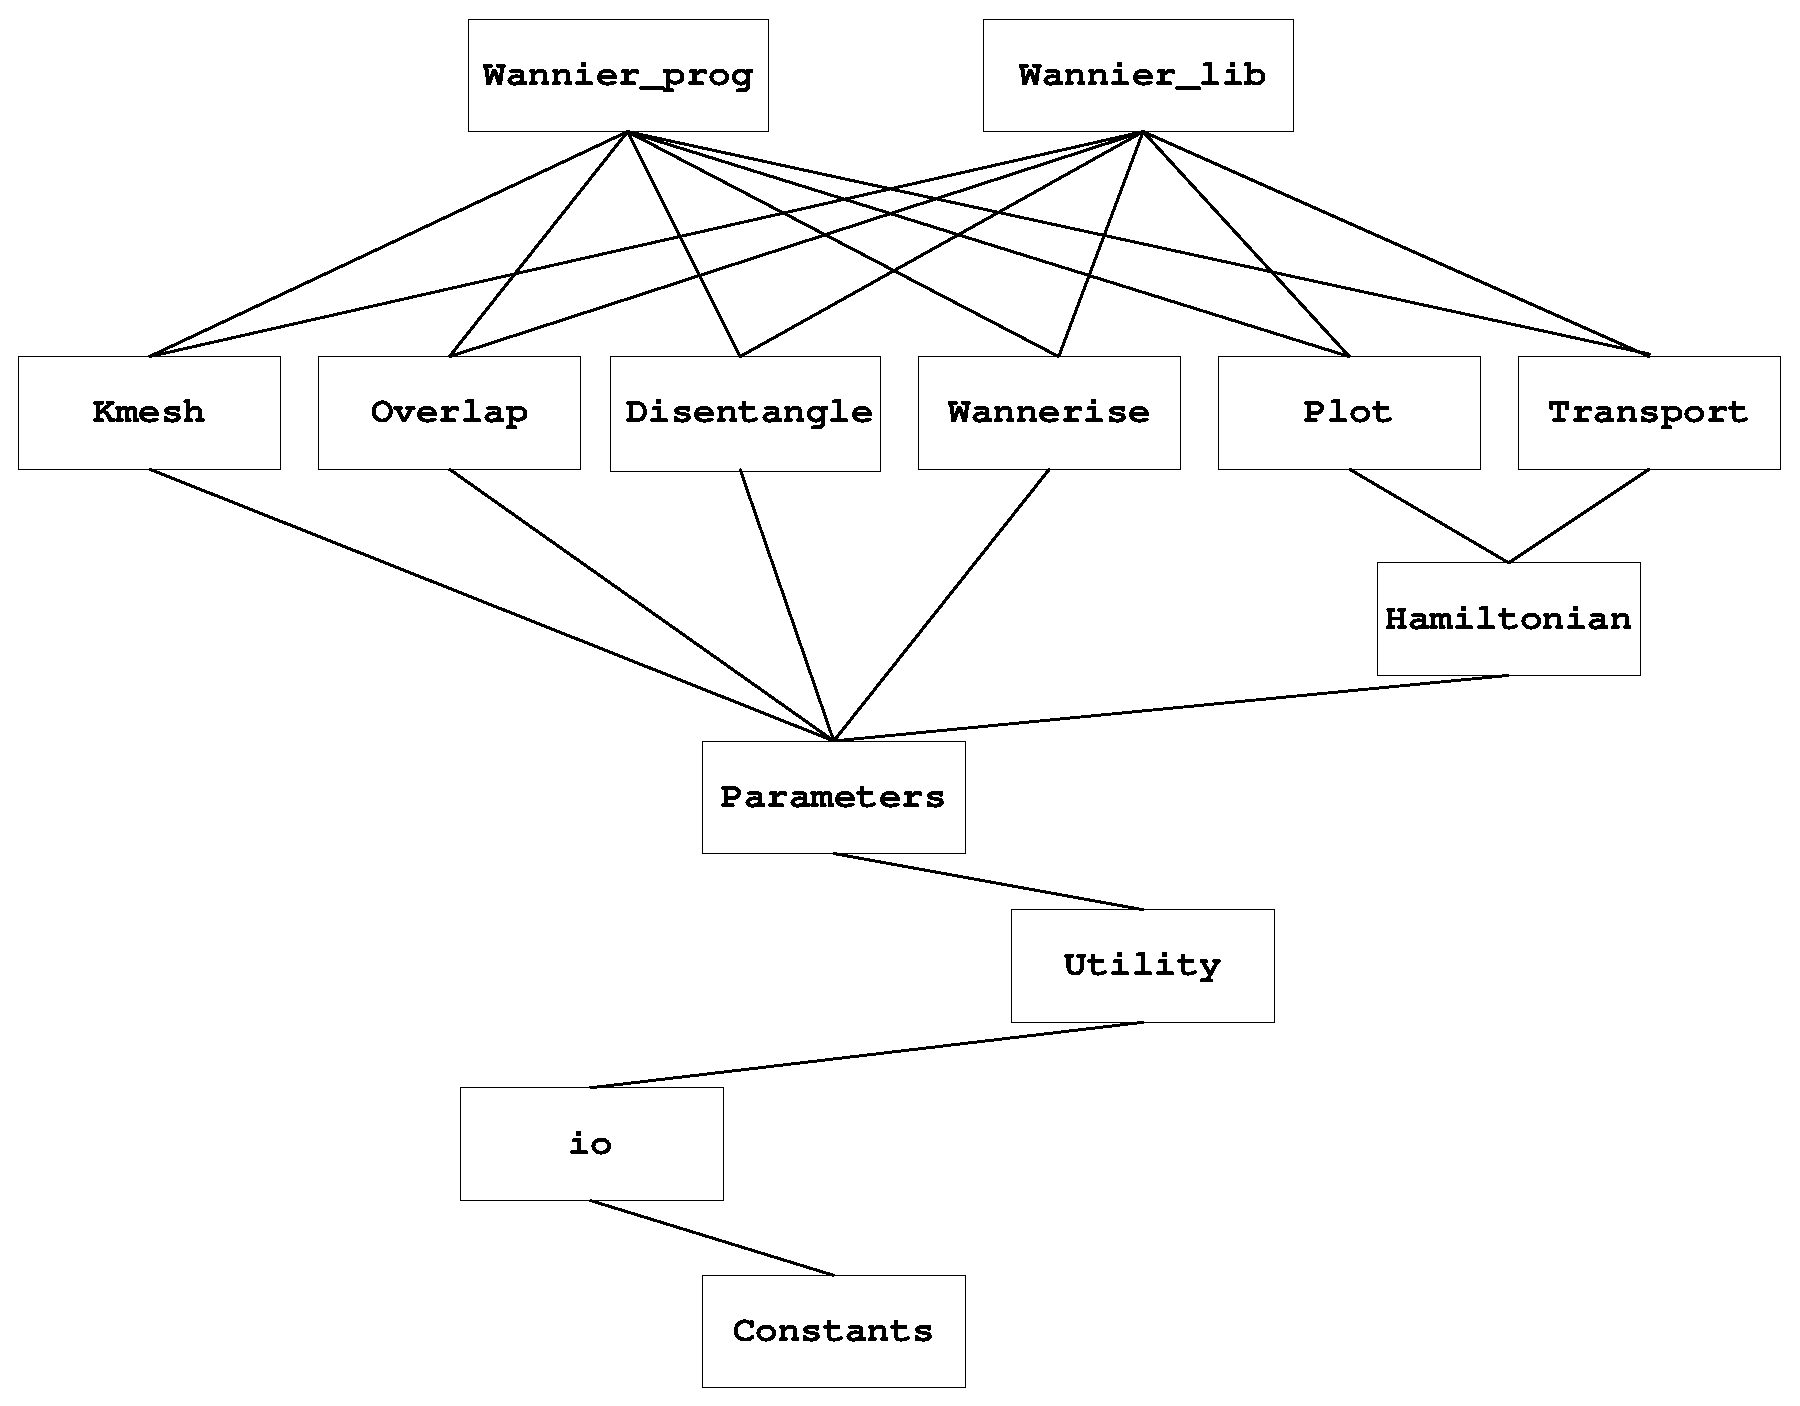
\includegraphics[width=5in]{overview}
\caption{Schematic overview of the module structure of
  \wannier. Modules may only use data and subroutines from lower
  modules.}
\label{structure}
\end{center}
\end{figure}
